% !TEX root = BRIR_measurements.tex

This document describes each of the rooms used to obtain the Binaural Room Impulse Responses (BRIRs) contained within this package and also the method used to obtain the anechoic responses.  Each of the rooms are described in a corresponding section of this document.  

The impulse responses were captured using a Cortex Instruments Mk.2 Head and Torso Simulator (HATS).  They were obtained from sinesweeps replayed through a Genelec 8020A active loudspeaker and the responses were deconvolved to produce the impulse responses. The recordings were made at a sampling frequency of 48 kHz (and subsequently resampled to 16 kHz).  The loudspeaker was placed around the HATS on an arc in the median plane with a 1500 mm radius between $\pm90^\circ$ and measured at $5^\circ$ intervals. The acoustic centre of the loudspeaker was placed at the same height as the ears.  A summary of the acoustical propoerties of each of the rooms is provided in \autoref{tab:RoomAcousticProps}. Measurements of \RT{} were obtained according to BS EN ISO 3382: 2000 using an interrupted pink noise method with six microphone positions and two loudspeaker positions (12 measurements in total).  In accordance with the standard, the overall room \RT{} is calculated by averaging the 500 Hz and 1 kHz bands. Other parameters were measured post-hoc directly from the impulse responses.

\begin{table}[t]\centering
\caption[Room acoustical properties]{Room acoustical properties, including \RT{}, Initial Time Delay Gap (ITDG), Direct-to-Reverberant Ratio (DRR) and clarity index C$_{\text{te}}$.}
{\footnotesize
\begin{tabular}{l r@{.}l r@{.}l r@{.}l r@{.}l}
\hline
\hline
\colheading{Room} & \multicolumn{2}{l}{\colheading{\RT{} [s]}} & \multicolumn{2}{l}{\colheading{ITDG [ms]}} & \multicolumn{2}{l}{\colheading{DRR [dB]}} & \multicolumn{2}{l}{\colheading{$\mathbf{C_{te}}$ (50 ms) [dB]}}\\\\
\hline
A & 0&32 & 8&72 & 6&09 & 16&5\\ % Our office 10bNC01
B & 0&47 & 9&66 & 5&31 & 11&4\\ % 07AC03
C & 0&68 & 11&9 & 8&82 & 17&4\\ % MS LT 03MS01
D & 0&89 & 21&6 & 6&12 & 9&43\\ % SeedPod 07NC01
\hline
\hline
\end{tabular}
}
\label{tab:RoomAcousticProps}
\end{table}

\section{Anechoic Condition}

For the anechoic condition, a pseudo-anechoic method was utilised whereby the responses were captured in a large room and simply truncated to before the first reflection so that subsequent reflections did not colour the frequency reponse.  The room measured $17.04 \times 14.53 \times 6.5$ m ($l \times w \times h$), the HATS and loudspeaker were placed in the centre of the room at a height of 2.8 m and separated by 1.5 m.  An example of this approach is shown in \autoref{fig:pseudo-anechoic} which was captured in the same space using a Genelec 8020A loudpseaker and a B\&K 4003 omnidirectional microphone at the same positions. It shows the captured impulse response (panel \subref{fig:pseudo-anechoic-IR}) and frequency responses calculated using both the full impulse response and the impulse response truncated to before the first reflection indicated at about 10 ms (panel \subref{fig:pseudo-anechoic-TF}).  It is clear that much of the frequency colouration has been removed.

\begin{figure}
\centering
	\begin{subfigure}{5.3in}
		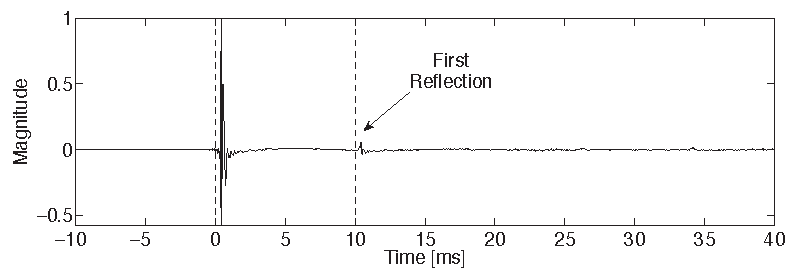
\includegraphics[width=5.3in]{pseudo-anechoic-IR}
		\caption[Impulse Response]{}\label{fig:pseudo-anechoic-IR}
		\vspace{2ex}
	\end{subfigure}
\\
	\begin{subfigure}{5.3in}
		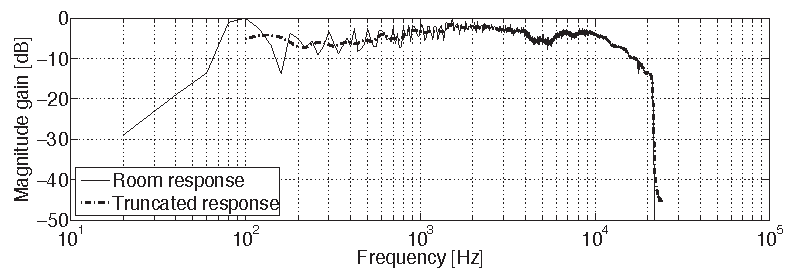
\includegraphics[width=5.3in]{pseudo-anechoic-TF}
		\caption[Frequency Response]{}\label{fig:pseudo-anechoic-TF}
	\end{subfigure}
\caption[Example of a pseudo-anechoic impulse response measurement]{Example of a pseudo-anechoic impulse response measurement.
(\subref*{fig:pseudo-anechoic-IR})~Impulse response captured in a large room.
(\subref*{fig:pseudo-anechoic-TF})~Frequency response of the truncated and un-truncated impulse responses.} 
\label{fig:pseudo-anechoic}
\end{figure}

\section{Room A}

Room A was a typical medium-sized office that seats 8 people but had surprisingly small \RT{} for its size.  The room layout and dimensions are given in \autoref{fig:RoomA}.



\section{Room B}

Room B was a medium--small class room.  Despite the small shoebox shape, the construction of the room gave it a relatively long \RT{} for its size.  The room layout and dimensions are given in \autoref{fig:RoomB}.



\section{Room C}

Room C was a large cinema--style lecture theatre that seats 418 people.  However, the abundance of soft seating and the low ceiling of the area around the lectern resulted in a relatively small \RT{} for the room's size.  The room layout and dimensions are given in \autoref{fig:RoomC}.



\section{Room D}

Room D was a typical medium--large sized seminar and presentation space with a very high ceiling.  The room layout and dimensions are given in \autoref{fig:RoomD}.

\section*{Acknowledgements}

The author would like to thank Joshua Brooks and Laurent Simon for their assistance with capturing the enclosed set of impulse responses. This work was supported by the EPSRC.

\begin{figure}
\centering
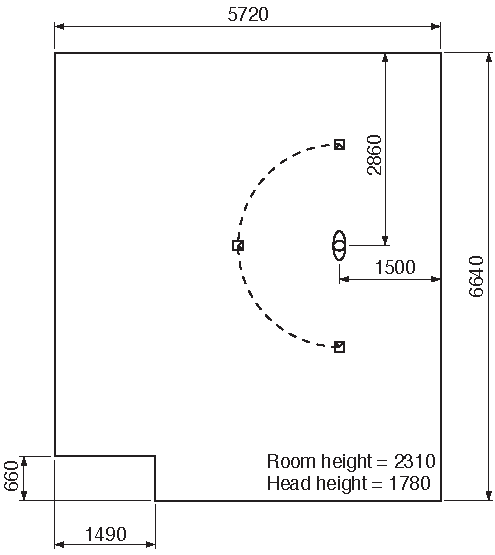
\includegraphics[width=3.3in]{Room_A}
\caption[Room A plan elevation]{Room A plan elevation and HATS location.}
\label{fig:RoomA}
\end{figure}

\begin{figure}
\centering
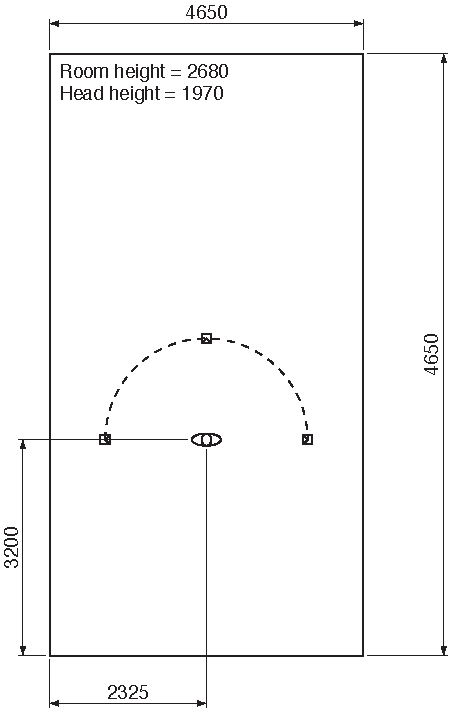
\includegraphics[width=3in]{Room_B}
\caption[Room B plan elevation]{Room B plan elevation and HATS location.}
\label{fig:RoomB}
\end{figure}

\begin{figure}
\centering
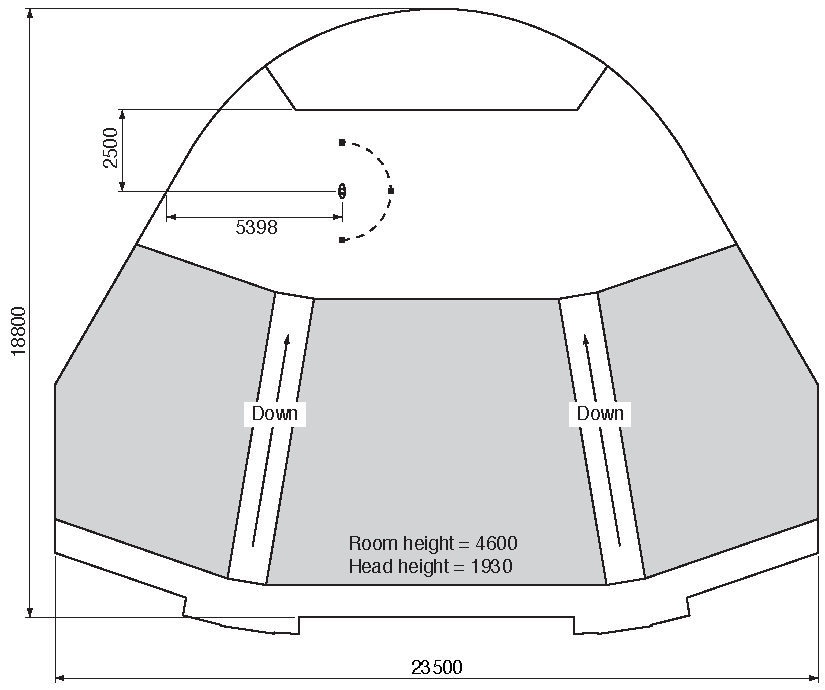
\includegraphics[width=5.5in]{Room_C}
\caption[Room C plan elevation]{Room C plan elevation and HATS location.  The shaded area denotes banked seating; the room height is the height of the room at the HATS position}
\label{fig:RoomC}
\end{figure}

\begin{figure}
\centering
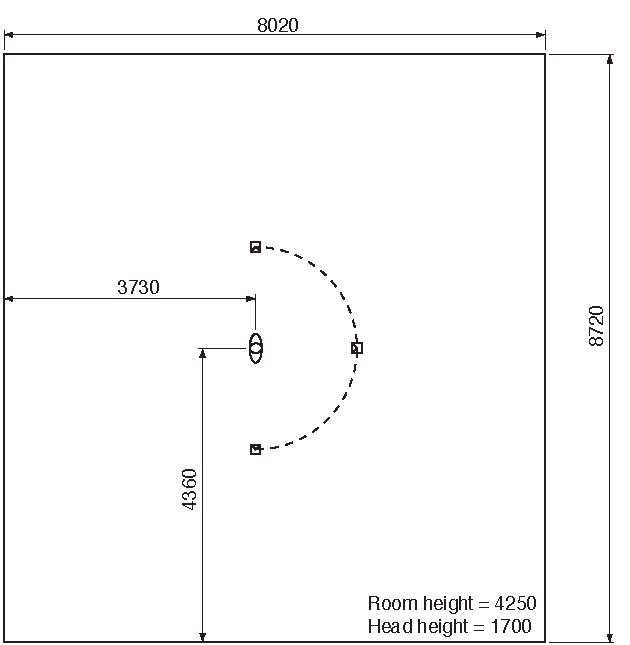
\includegraphics[width=4.2in]{Room_D}
\caption[Room D plan elevation]{Room D plan elevation and HATS location.}
\label{fig:RoomD}
\end{figure}